%
% sinh.tex -- warum sinh und cosh für gewöhnliche DGl so nützlich sind XXX
%
% (c) 2015 Prof Dr Andreas Müller, Hochschule Rapperswil
%
\chapter{Hyperbolische Funktionen}
Das Standardverfahren für die Lösung linearer Differentialgleichungen
mit konstanter Koeffizienten liefert typischerweise Schwingungslösungen
oder exponentiell abfallende oder anwachsende Lösungen. Die Koeffizienten
der allgemeinen Lösungen müssen dann mit Hilfe der Anfangswerte bestimmt
werden. Für die Schwingunsglösungen ist das meist sehr viel einfacher
als für die exponentiellen Lösungen. Hier wird gezeigt, wie man mit
Hilfe der hyperbolischen Funktionen die Lösungen ebenso einfach ausdrücken
kann.

%
% ode.tex -- XXX
%
% (c) 2019 Prof Dr Andreas Müller, Hochschule Rapperswil
%
\section{Differentialgleichungen zweiter Ordnung}
Das Standardverfahren für die Lösung einer gewöhnlichen linearen
Differentialgleichung mit konstanten Koeffizienten
\[
a_2y''+ a_1y'+a_0y=0
\]
schreibt vor, dass man erst die Nullstellen $\lambda_{1,2}$
des charakteristischen Polynoms
\[
p(\lambda)=a_2\lambda^2+a_1\lambda+a_0
\]
finden muss.
Die allgemeine Lösung der Differentialgleichung ist dann
eine Linearkombination
\[
y(x)=
A_1 e^{\lambda_1t}
+
A_2 e^{\lambda_2t},
\]
die Konstanten $A_1$ und $A_2$ sind aus den Anfangswerten zu bestimmen.
Sinde $y_0$ und $v_0$ der Anfangswert und die Anfangsableitung, dann
findet man das lineare Gleichungssystem
%\newcolumntype{\linsysR}{>{$}r<{$}}
%\newcolumntype{\linsysL}{>{$}l<{$}}
%\newcolumntype{\linsysC}{>{$}c<{$}}
%\newenvironment{linsys}[1]{%
%\begin{tabular}{*{#1}{\linsysR@{\;}\linsysC}@{\;}\linsysR}}%
%{\end{tabular}}
\[
\begin{linsys}{3}
         A_1&+&         A_2&=&y_0\phantom{.}\\
\lambda_1A_1&+&\lambda_2A_2&=&v_0.
\end{linsys}
\]
Besonders einfach wird die Bestimmung jedoch für die Differentialgleichung
\[
y''+k^2 y=0.
\]
Dann sind die $\lambda_{1,2}=\pm\sqrt{-k^2}$ imaginär, und man kann statt
der Exponentiallösungen auch den Ansatz
\[
y(x)=A\cos kx+B\sin kx
\]
verwenden.
Da der Wert von $\sin kx$ bei $x=0$ verschwindet, und die Ableitung von
$\cos kx$ ebenfalls, ist die Bestimmung der Konstanten viel einfacher:
\[
A=y_0
\qquad\text{und}\qquad
B=\frac1kv_0,
\]
oder
\begin{equation}
y(x)=y_0\cos kx + \frac{v_0}{k}\sin kx
\label{hyp:loesung}
\end{equation}

Für die analoge Differentialgleichung $y''-k^2y=0$ geht dies nicht.
Die Nullstellen des charakteristischen Polynoms sind hier 
$\lambda_{1,2}=\pm k$, und es führt nichts an dem linearen Gleichungssystem
\[
\begin{linsys}{3}
 A_1&+& A_2&=&y_0\\
kA_1&-&kA_2&=&v_0
\end{linsys}
\]
vorbei.
Die Lösung kann allerdings zum Beispiel mit dem Determinantenverfahren
ziemlich direkt gefunden werden:
\begin{align*}
A_1
&=
\frac{\left|\begin{matrix}y_0&1\\v_0&-k\end{matrix}\right|}{\left|\begin{matrix}1&1\\k&-k\end{matrix}\right|}
=
\frac{-ky_0+v_0}{-2k},
&
A_2
&=
\frac{\left|\begin{matrix}1&y_0\\k&v_0\end{matrix}\right|}{\left|\begin{matrix}1&1\\k&-k\end{matrix}\right|}
=\frac{v_0-ky_0}{-2k}.
\end{align*}
Damit kann man jetzt die Lösung auch in diesem Fall hinschreiben:
\begin{align}
y(x)
&=
A_1e^{kx}+A_2e^{-kx}
=
\frac12\biggl(
\frac{ky_0-v_0}k e^{kx}
+
\frac{-v_0+ky_0}k e^{-kx}
\biggr)
\notag
\\
&=
y_0\frac{e^{kx}+e^{-kx}}2
+\frac{v_0}{k}\frac{e^{kx}-e^{-kx}}2.
\label{hyp:hyperbelfunktionen}
\end{align}
Die Erfüllung der Anfangsbedingung könnte also auch in diesem Falle
sehr einfach sein, wenn man nicht die Funktionen $e^{\pm kx}$ verwenden
würde, sondern deren Linearkombinationen wie in (\ref{hyp:hyperbelfunktionen}).


%
% hyp.tex -- 
%
% (c) 2015 Prof Dr Andreas Müller, Hochschule Rapperswil
%
\section{Hyperbolic functions}
\lhead{Hyperbolic functions}
\begin{figure}
\centering
%\includegraphics{../common/images/hf-1.pdf}
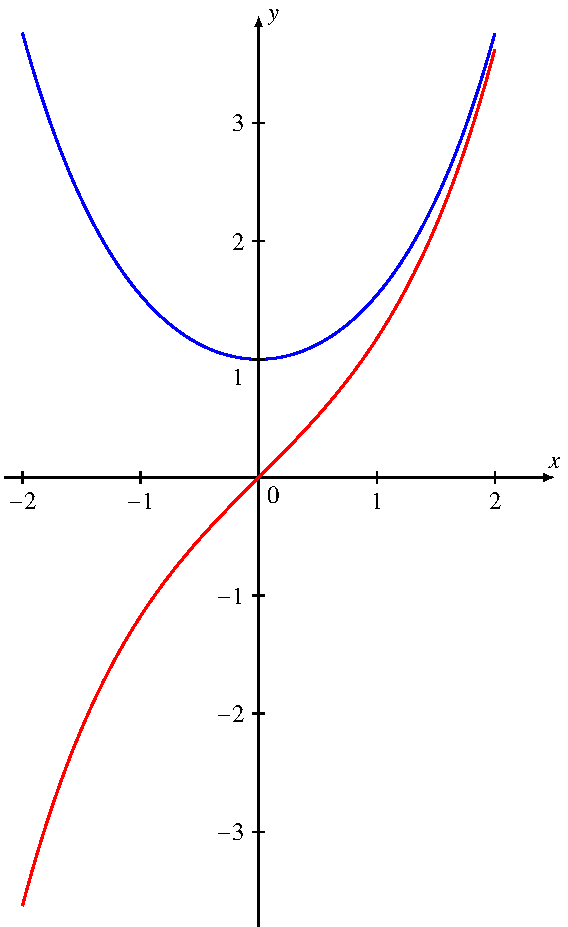
\includegraphics{b-sinh/images/sinhcosh.pdf}
\caption{Graphs of the functions 
$x\mapsto\cosh x$ (blue)
and $x\mapsto\sinh x$ (red)
\label{hyp:graphen}}
\end{figure}
The hyperbolic function are defined as
\[
\sinh x =\frac{e^x-e^{-x}}2
\qquad\text{and}\qquad
\cosh x = \frac{e^x+e^{-x}}2.
\]
Figure~\ref{hyp:graphen} shows graphs of those two functions.
At first sight these definitions have nothing to do with trigonometric
functions, the names {\em sinus hyperbolicus} for $\sinh x$ and
{\em cosinus hyperbolicus} for $\cosh x$ seem unjustified.

\subsection{Complex definition of the trigonometric functions}
From the Euler-formula
\[
e^{it}=\cos t+i\sin t
\]
a complex definition for the trigonometric functions can be derived
as follows.
Using the Euler-formula for $t$ and $-t$ we get
\begin{align*}
\cos t+i\sin t&=e^{it}\\
\cos t-i\sin t&=e^{-it}.
\end{align*}
This is a system of linear equations which can be solved
for the functions $\cos t$ and $\sin t$ using the addition method.
We find
\begin{align*}
\cos t
&=
\frac{e^{it}+e^{-it}}2
&
\sin t
&=
\frac{e^{it}-e^{-it}}{2i}.
\end{align*}
The trigonometric functions can thus be defined in a way very similar
to the hyperbolic functions.
The only difference is a factor $i$ here and there.
Thus it is reasonable to expect that the hyperbolic functions
have many properties completely analogous to properties of the
trigonometric functions, with may be a sign change here and there.

\subsection{Geometry}
The trigonometric functions stem from the desire to compute right
triangles.
More precisely, the trigonometric functions compute right triangles
where one side has length $1$.
This is usually illustrated by identifying the values of the
trigonometric functions as line segments in a unit circle.
This is possible thanks to the well known identity
\[
\sin^2t+\cos^2t=1
\]
which implies that the function
\[
t\mapsto (\cos t,\sin t)
\]
parametrizes the unit circle.

\begin{figure}
\centering
%\includegraphics{../common/images/hf-2.pdf}
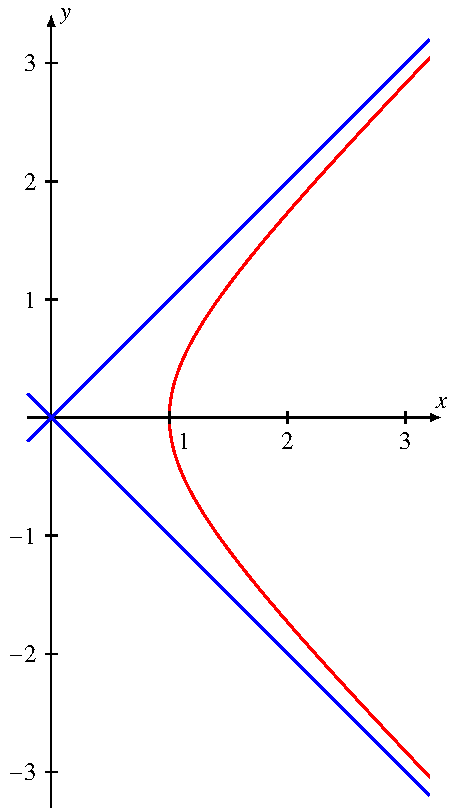
\includegraphics{b-sinh/images/hyperbola.pdf}
\caption{The curve with the parametrization
$t\mapsto (\cosh t, \sinh t)$ is a ``unit hyperbola'' (red) with 
asymptotes
$y=\pm x$ (blue).
\label{anhang:hyperbel}}
\end{figure}
The hyperbolic functions define a map
\[
t\mapsto (\cosh t, \sinh t)
\]
which is of course in the plane.
To find out what type of curve this could be, we compute the
squares of these functions:
\begin{align}
\sinh^2 t&=\frac14(e^{2t}-2+e^{-2t}),
\\
\cosh^2 t&=\frac14(e^{2t}+2+e^{-2t}).
\label{hyp:definition}
\end{align}
Up to the middle term, the are identical.
Their difference is
\[
\cosh^2t - \sinh^2t=1,
\]
so the hyperbolic functions describe a curve with the equation
\[
x^2-y^2=1.
\]
This is a hyperbola with asymptotes $y=\pm x$
(figure~\ref{anhang:hyperbel}).
This justifies that we call these functions hyperbolic functions.

\subsection{Addition theorems}
Is there an addition formular for hyperbolic functions?
If the analogy to trigonometric functions works, we would expect 
formulae like
\begin{align*}
\sinh(a+b)&=\sinh a\cosh b + \cosh a\sinh b,\\
\cosh(a+b)&=\cosh a\cosh b - \sinh a\sinh b,
\end{align*}
with some different signs here and there.
To verify this, we use the definition and compute
\begin{align*}
\sinh a\cosh b + \cosh b\sinh b
&=
\frac14(e^a-e^{-a})(e^b+e^{-b})
+
\frac14(e^a+e^{-a})(e^b-e^{-b})
\\
&=\frac14(e^{a+b}+e^{a-b}-e^{-a+b}-e^{-a-b} + e^{a+b}-e^{a-b}+e^{-a+b}-e^{-a-b})
\\
&=
\frac14(2e^{a+b}-2e^{-a-b})
=
\frac12(e^{a+b}-e^{-a-b})=\sinh(a+b),
\\
\cosh a\cosh b-\sinh a\sinh b
&=
\frac14(e^a+e^{-a})(e^b+e^{-b})
-
\frac14(e^a-e^{-a})(e^b-e^{-b})
\\
&=
\frac14(e^{a+b}+e^{a-b}+e^{-a+b}+e^{-a-b})
-
\frac14(e^{a+b}-e^{a-b}-e^{-a+b}+e^{-a-b})
\\
&=
\frac14(2e^{a-b}+2e^{-a+b})
=
\frac12(e^{a-b}+e^{-a+b})=\cosh(a-b).
\end{align*}
The conjecture regarding the addition theorems was correct in the cause
of $\sinh(a+b)$, but for $\cos(a+b)$ we had to change a sign.
The correct form of the addition formulae is
\begin{align*}
\sinh(a\pm b)&=\sinh a\cosh b \pm \cosh a\sinh b,\\
\cosh(a\pm b)&=\cosh a\cosh b \pm \sinh a\sinh b.
\end{align*}

\subsection{Derivatives}
In analysis one learns to derive formulae for the derivatives of the
trigonomtric functions from the addition theorems.
Since the addition theorems for hyperbolic functions are so similar
up the a sign, the the rules for the derivatives should look just the
same, up to a sign.

We can also find the derivatives directly from the definition
\eqref{hyp:definition} by applying the derivation rules for the
exponential function:
\begin{align*}
\frac{d}{dx}\cosh x
&=
\frac12\frac{d}{dx}(e^x+e^{-x})
=
\frac12(e^x-e^{-x})=\sinh x
\\
\frac{d}{dx}\sinh x
&=
\frac12\frac{d}{dx}(e^x-e^{-x})
=
\frac12(e^x+e^{-x})=\cosh x
\end{align*}
Thus the derivatives are even simpler, as they start to repeat already
at the second derivative.
The second derivative already is the original function
\begin{align*}
\sinh''x&=\sinh x
&
\cosh''x&=\cosh x.
\end{align*}

\subsection{Values for argument $0$}
The values of the trigonometric functions and their first derivatives
at the origin and the respective values for the hyperbolic
functions also are very similar:
\begin{center}
\begin{tabular}{|l|>{$}c<{$}>{$}c<{$}|>{$}c<{$}>{$}c<{$}|}
\hline
Wert für $x=0$ von&\sin x&\cos x&\sinh x&\cosh x\\
\hline
Funktion           &  0   &  1   &   0   &   1   \\
Ableitung          &  1   &  0   &   1   &   0   \\
\hline
\end{tabular}
\end{center}

\subsection{Solving differential equations}
The values for argument $0$ are precisely the properties
that make satisfying the initial values of a differential 
equation so simple.
The differential equation
\[
y''-k^2y=0
\]
with initial conditions
\[
y(0)=y_0\qquad\text{and}\qquad y'(0)=v_0
\]
has solution
\[
y(x)=y_0\cosh kx +\frac{v_0}{k}\sinh kx,
\]
in complete analogy to
\eqref{hyp:loesung}.


